\documentclass[tikz]{standalone}
\usetikzlibrary{arrows.meta}
\begin{document}

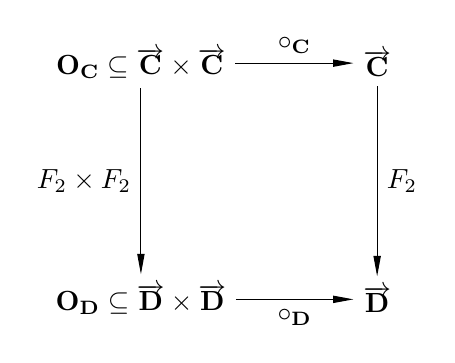
\begin{tikzpicture}[-latex, arrows={-Triangle[angle=20:5pt,scale=1.5]}]
	\node (A) at (0,0) {\(\mathbf{O} _{\mathbf{C}} \subseteq \overrightarrow{\mathbf{C}} \times  \overrightarrow{\mathbf{C}}\)};
	\node (B) at (3,0) {\(\overrightarrow{\mathbf{C}}\)};
	\node (C) at (0,-3) {\(\mathbf{O} _{\mathbf{D}}\subseteq \overrightarrow{\mathbf{D}} \times  \overrightarrow{\mathbf{D}}\)};
	\node (D) at (3,-3) {\(\overrightarrow{\mathbf{D}}\)};

	\draw (A) to node [above] {\(\circ _ \mathbf{C}\)} (B);
	\draw (A) to node [left] {\(F_2 \times F_2\)} (C);
	\draw (B) to node [right] {\(F_2\)} (D);
	\draw (C) to node [below] {\(\circ _ \mathbf{D}\)} (D);
\end{tikzpicture}

\end{document}
